\documentclass{article}

\usepackage{verbatim}
\usepackage{minted}
\usepackage{graphicx}
\usepackage[utf8]{inputenc}

\title{Langages synchrones : TP2}

% A rendre le 04/11
% Metronome: 1,2,3,6
% Arbitre McMillan: 1,2
% Extensions: Q1 (non determinism), Q2 (asynchronisme)

%ssh 3367424@ssh.ufr-info-p6.jussieu.fr

\author{I\~{n}igo Mediavilla \& Pierrick Couderc}

\begin{document}

\maketitle

\section{Métronome}


\subsection{Noeud Lustre}

\begin{verbatim}
node metronome (reset : bool; delay : int) 
     returns (tic, tac : bool);
  var n, hz : int;
      state, first, tmp: bool;
let
    hz = 0 -> if reset then delay - 1 else pre hz;
    n = 0 -> if reset then delay
             else if pre n = 0 and first then hz
             else (pre n) - 1;
    first = false -> reset or pre first;
    state = n = 0 and first;

    tmp = true -> if state then not pre tmp else pre tmp;
    
    tic = if state then tmp else false;
    tac = if state then not tmp else false;
tel
\end{verbatim}


In the figure~\ref{trace-metronome-1} we can see how the given code
emulates the behaviour of the metronome. In the step 6, we set a
delay of 1 and we verify that the metronome emits tics and tacs
alternatively. In the step 13 we modify the delay to 5 and we not
only see how this delay is respected but also how the next signal
emitted is not tic but tac, since the last sinal emmited with delay
1 was tic.

\begin{figure}[!ht]
\label{trace-metronome-1}
\caption{Execution of the metronome}
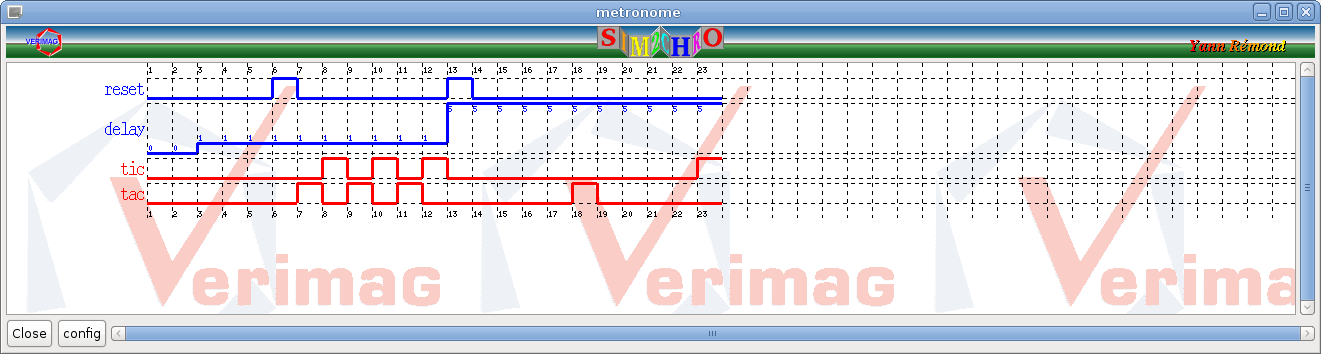
\includegraphics [width=1.2\textwidth, natwidth=750,natheight=600]{metronome_1.png}
\end{figure}

\subsection{Automaton}

The code for C for the metronome that is generated with the commands
lus2oc and poc is shown in figure~\ref{metronome-0}.

The correspondance of the variables in the C code with
respect to the code in lustre is the following:

\begin{itemize}
\item V1 = reset
\item V2 = delay
\item V3 = initial state = false
\item V4 = n              
\item V5 = first         
\item V6 = hz
\item V7 = tmp               
\item V8 = tic  
\item V9 = tac
\item V10 = state
\end{itemize}


\begin{figure}[ht]

\begin{minted}[mathescape,
               linenos,
               numbersep=5pt,
               gobble=2,
               frame=lines,
               framesep=2mm]{c}
  switch(ctx->current_state){
   case 0:
      ctx->_V5 = (ctx->_V3? _false : (ctx->_V1 || ctx->_V5));
      ctx->_V6 = (ctx->_V3? 0 : (ctx->_V1? (ctx->_V2 - 1) : ctx->_V6));
      ctx->_V4 = (ctx->_V3? 0 : (ctx->_V1? ctx->_V2 : (((ctx->_V4 == 0) &&
   ctx->_V5)? ctx->_V6 : (ctx->_V4 - 1))));
      ctx->_V10 = ((ctx->_V4 == 0) && ctx->_V5);
      ctx->_V7 = (ctx->_V3? _true : (ctx->_V10? (!ctx->_V7) : ctx->_V7));
      ctx->_V3 = _false;
      ctx->_V8 = (ctx->_V10? ctx->_V7 : _false);
      metronome_O_tic(ctx->client_data, ctx->_V8);
      ctx->_V9 = (ctx->_V10? (!ctx->_V7) : _false);
      metronome_O_tac(ctx->client_data, ctx->_V9);
      ctx->current_state = 0; break;
   break;
   } /* END SWITCH */
\end{minted}
\label{metronome-0}
\caption{Code C generated with with lus2oc -0 and poc}
\end{figure}


And thus the corresponding automaton for the C code is shown
in figure~\ref{automaton-0}

\begin{figure}[ht]
\begin{center}
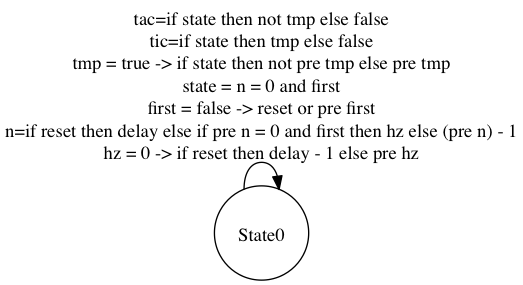
\includegraphics[width=0.8\textwidth, natwidth=610,natheight=642] {automaton-0.png}
\end{center}
\label{automaton-0}
\caption{Automaton without unfolding}
\end{figure}

If we generate the automaton with the option -2, the automaton
is unfolded so the only state that we had for the option -0, is
converted into 4 states. As demonstrated by figure~\ref{automaton-2}
the automaton is unfolded based on the values of the signals \emph{reset}
and \emph{state}.

\begin{figure}[ht]
\label{automaton-2}
\caption{Automaton with unfolding}
\begin{center}
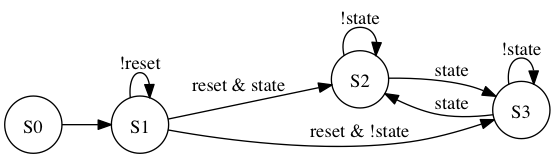
\includegraphics[width=0.8\textwidth, natwidth=610,natheight=642]{automaton-2.png}
\end{center}
\end{figure}


\subsection{Verification}

\begin{itemize}

\item P1: At every moment there cannot be a tic and a tac simultaneously

\begin{verbatim}
node not_same_time(tic, tac:bool) returns (out: bool)
let
  out = not (tic and tac);
tel
\end{verbatim}

\item P2: There can never be two consecutive tics 

\begin{verbatim}

node not_tic_after_tic(tic, tac:bool) returns (out:bool)
let
  out = once_from_to(tac, tic, tic);
tel

node once_from_to (X, A, B : bool) returns (ok : bool)
var x_after_a, s: bool;
let
  x_after_a = false -> if pre B then false
                       else if s and X then true
                       else if pre x_after_a and A then false
                       else pre x_after_a;

  s = switch (false, A, B);

  ok =  true ->

  if s then true else if B and not x_after_a then false else pre ok;
tel

node switch (orig, on, off : bool) returns (state : bool);
let

  state = orig -> if on then true

  else if off then false

  else pre state;
tel

\end{verbatim}

\item P3: The delay between two tics must be equal to twice the delay
  given in the last reset unless a reset happens between the two tics.

We haven't managed to make it validate on xlesar, even though the
following code seemed to give reasonable results when tracing it with
luciole as shown in the following figure.


\begin{verbatim}
node obs3 (tic, reset : bool; delay : int) returns (out: bool)
   var twice_last, last_delay, last_tic : int; counting: bool;
let
   assert (delay > 1);
   last_delay = delay -> if reset then delay else pre last_delay;
   last_tic =  0 -> if tic then 0
                    else if counting then (pre last_tic) + 1
                    else 0;
   counting = false -> if reset and not tic then false
              else if tic then true
              else pre counting;
   twice_last = (pre last_delay * 2);
   out = true -> if tic and (pre counting) then 
                   twice_last = ((pre last_tic) + 1) else true;
tel
\end{verbatim}

\begin{figure}[!ht]
\begin{center}
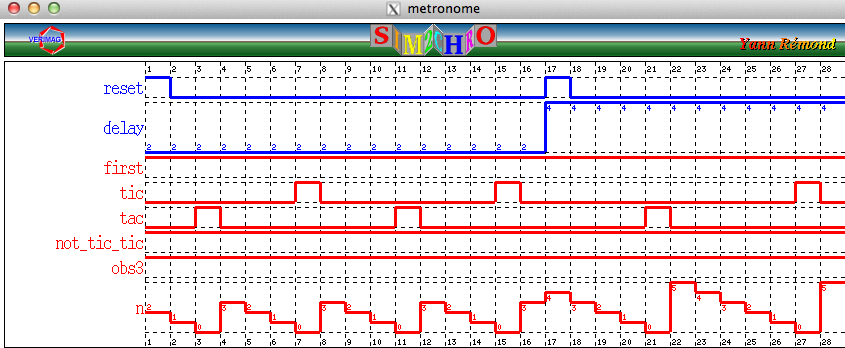
\includegraphics[width=0.8\textwidth, natwidth=610,natheight=642] {img/trace-obs3.png}
\end{center}
\label{trace-obs3}
\caption{Tracing P3 with luciole}
\end{figure}

\end{itemize}

\section{Modeling a bus arbitration system}

\subsection{Noeud Lustre}

\begin{verbatim}

node cellule(token_in, req_in, grant_in, ovr_in:bool) 
  returns (token_out, grant_out, ovr_out, ack_out : bool)
  var tmp_ovr2, tmp_ovr3 : bool;
let
  token_out = false -> (pre token_in);

  tmp_ovr2 = false -> (req_in and ((pre token_in) or (pre tmp_ovr2)));
  tmp_ovr3 = false -> ((pre token_in) and pre tmp_ovr2);
  ovr_out = ovr_in or tmp_ovr3 ;

  grant_out = (not req_in) and grant_in;

  ack_out = (grant_in or tmp_ovr3) and req_in;
tel

node mcmillan(req_in_1, req_in_2, req_in_3: bool)
   returns (ack_out_1, ack_out_2, ack_out_3: bool)
   var tk_out_1, tk_out_2, tk_out_3,
       gr_out_1, gr_out_2, gr_out_3,
       ovr_out_1, ovr_out_2, ovr_out_3: bool;
let
   (tk_out_1, gr_out_1, ovr_out_1, ack_out_1) = 
         cellule(true -> tk_out_3, req_in_1, gr_out_2, false);
   (tk_out_2, gr_out_2, ovr_out_2, ack_out_2) = 
         cellule(tk_out_1, req_in_2, gr_out_3, ovr_out_1);
   (tk_out_3, gr_out_3, ovr_out_3, ack_out_3) = 
         cellule(tk_out_2, req_in_3, false -> not ovr_out_3, ovr_out_2);
tel
\end{verbatim}

\subsection{Functioning}

In the bus the cells have different priority level with 3 having the higher 
priority and cell 1 the lower.

When two cells request access to the bus, the one that has the priority gets the
ack. However the arbitration system provides a mechanism to avoid a request waiting forever that 
is based on a token. A token is a signal that passes from one cell to the following
starting by cell1 and that avoids the deadlock because a cell that gets request
access to the bus for long enough to get twice the token, is automatically granted
access as soon as it gets the token the second time.

We can see how this mechanism applies practically with the following examples:

\begin{itemize}

\item When there's only one of them that is requesting then it gets the ack all 
the time.

\begin{figure}[!ht]
\begin{center}
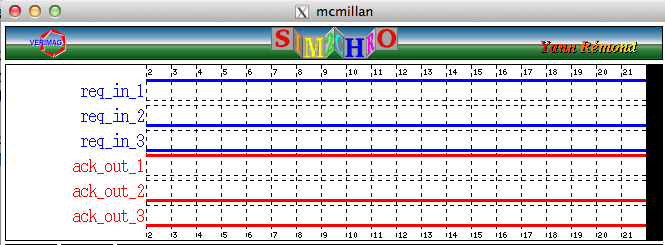
\includegraphics[width=0.8\textwidth, natwidth=610,natheight=642] {img/all-req-1.png}
\end{center}
\label{all-req-1}
\caption{Arbitration for a single continous request}
\end{figure}

\item When there's two that request separately, they don't conflict so the one that
demands always get the ack

\begin{figure}[!ht]
\begin{center}
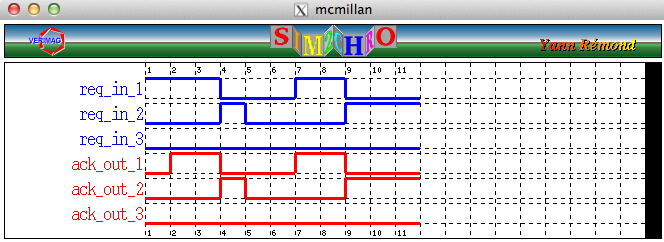
\includegraphics[width=0.8\textwidth, natwidth=610,natheight=642] {img/two-alternative-req.png}
\end{center}
\label{two-alternate-req}
\caption{Arbitration for two alternative requests}
\end{figure}


\item When there's two of them that request continuosly, then one gets two turns and 
the other gets one turn out of three

\begin{figure}[!ht]
\begin{center}
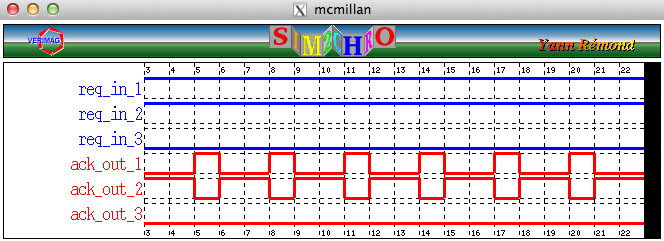
\includegraphics[width=0.8\textwidth, natwidth=610,natheight=642] {img/two-continuosly.png}
\end{center}
\label{two-continuosly}
\caption{Arbitration for two continuos requests}
\end{figure}

\item When there are three requests at the same time, the third cell always takes the
ack because it has priority over the others and since no cell keeps the request
long enough to get twice the token while the request is active, the mechanism to avoid
deadlock doesn't activate.

\begin{figure}[!ht]
\begin{center}
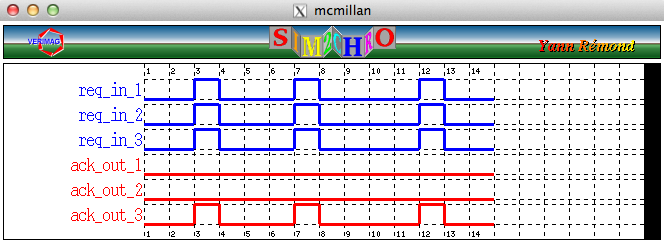
\includegraphics[width=0.8\textwidth, natwidth=610,natheight=642] {img/three-sporadic.png}
\end{center}
\label{three-sporadic}
\caption{Arbitration for three sporadic requests}
\end{figure}

\item When there's three continuosly that have been waiting waiting for more than one cycle
for the token, the graph shows that the three get the ack alternatively. Every time 
  one gets the ack is because it's because that cell is getting the token

\begin{figure}[!ht]
\begin{center}
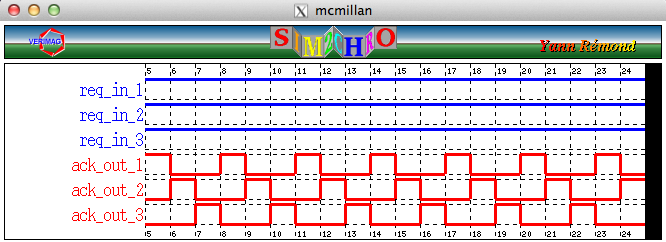
\includegraphics[width=0.8\textwidth, natwidth=610,natheight=642] {img/three-continuosly.png}
\end{center}
\label{three-continuosly}
\caption{Arbitration for three continuous requests}
\end{figure}

\item In the beginning we can see that the first time we don't have enough info
to calculate the acks so we return false by default even though the three
acks have been activated. The token initially is in cell 1. On the second, third
and fourth steps cell 3 gets the ack because it has priority with respect to cells 
1 and 2. Finally they get back to the behaviour of alternating the ack shown in the
previous example.
 
\begin{figure}[!ht]
\begin{center}
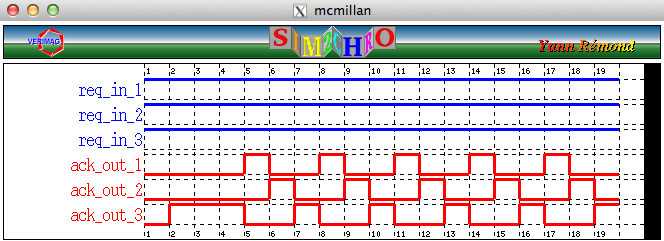
\includegraphics[width=0.8\textwidth, natwidth=610,natheight=642] {img/three-continuosly-from-beginning.png}
\end{center}
\label{three-continuosly-from-beginning}
\caption{Arbitration for three continuous requests from the beginning}
\end{figure}

\end{itemize}

\subsection{McMillan's referee - Automaton}

When generating the automaton with lus2oc and the code with poc we can see how
the code contains 24 states. Every change to a new state is guided by the input
signals req\_in\_1, req\_in\_2 and req\_in\_3. Intuitively we can imagine that
the states have been unfolded based on whether the cells have been waiting for
an ack since the last time they got the token or not and if they have the token
now or not. We can see that if at every step we need to keep for every cell
a boolean value saying if the cell has been waiting for the ack since the last
token then we need $2^{3}$ states just to do that. If on top of that we need
to keep track on where the token is at every moment we need to multiply the 
previous value by three (the token can be in cell1, cell2 or cell3) what
gives us the value of 24 $2^{3}~\times~4~=~24$.

\section{Modélisation de systèmes indéterminisites et/ou asynchrones}

\subsection{Indéterminisme}

If we suppose the constraints given, we can modelize the following node :

\begin{verbatim}
node env(S,R : bool; o : bool) returns (set,reset : bool);
let
  set = if S and not R then true
        else if S and R then o
             else false;
  reset = if R and not S then true
          else if S and R then not o
               else false;
tel
\end{verbatim}

\paragraph{Question 1} 

We can easily prove that the node follows the constraints
by verifying the property $not~(set~ and~ reset)$ in xlesar, which will return
\emph{True property}. However, it isn't enough to prove that it can give any
(and every, not in the same time of course) of the other patterns. We can easily
prove that it will be the case, whatever the oracle's value is.

First, if we consider S and R false, then reset will be false and set too. If
S is true and R false, then set will be true and reset false. The symetrical
equivalent will give the symetrical result. The last case will be S and R as
true, which will give respectively the value of the oracle and its contrary.

\paragraph{Question 2} 

To verify the first property, we could give an observer \\
 ($assert(not~(set~ and~reset))$), however the second one (the node can give every of the other
patterns) can't be verified with one, except if we ``register'' each incoming
pattern and result associated  and once we have all of them (excluding the
oracle), verify that we had $<set=0, reset=0>$, $<set=1, reset=0>$ and $<set=0,
reset=1>$, which is kind of complicated.

\subsection{Asynchronisme}

\paragraph{Question 1}

We can easily extend the scheduler by adding the construction from activ\_C:

\begin{verbatim}
node main(x,y : int; S, R : bool) returns (o1,o2 : int);
let
        o1 = current(C1(x when S));
        o2 = current(C2(y when R));
tel
\end{verbatim}

This way, we get the value from C1 (or C2) only when we give S (respectively R),
otherwise the previous value is given.

\paragraph{Question 2}

The graph representing the following asynchronous node:

\begin{center}
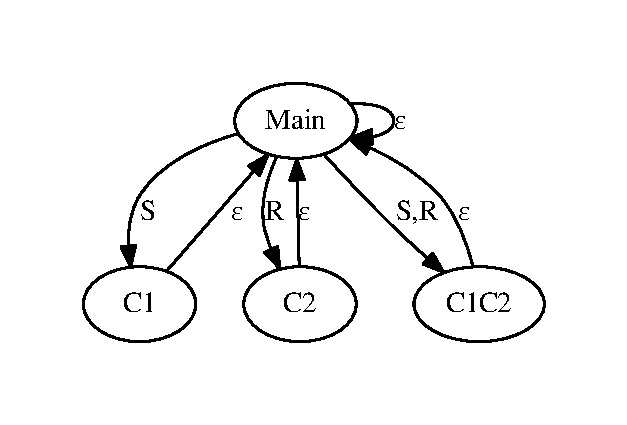
\includegraphics{asyn_1.pdf}
\end{center}

Since C1 and C2 are totaly independant, they don't have interaction. Moreover,
we don't need their behavior and can suppose they are simply a state. We add
another state, \emph{C1C2}, which correspond to the possibility of having C1 and
C2 executed at the same time, and an $\epsilon$-transition from Main to Main,
corresponding of no activation at all.

\paragraph{Question 3}

We can add strict asynchronism on the scheduler by reusing the env node from the
previous part. This way, we can assure the at most one component can activate,
since the variable set and reset can't be true at the same time.

\begin{verbatim}
node main(x,y : int; S, R : bool) returns (o1,o2 : int);
let
        set, reset = env(S, R, true);
        o1 = current(C1(x when set));
        o2 = current(C2(y when reset));
tel
\end{verbatim}

The following state graph is then:

\begin{center}
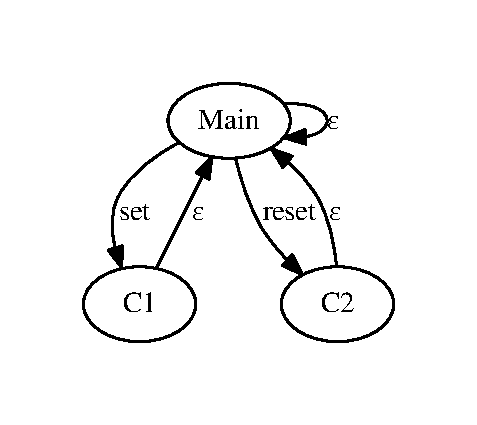
\includegraphics{asyn_strict.pdf}
\end{center}

The result is obvious, since we just need to remove the \emph{C1C2} part from
the graph.


\end{document}
